% !TEX root = ../main.tex

% 中英标题:\chapter{中文标题}[英文标题]

\chapter{基于无配对数据的初步声纳去噪}

\section{引言}[Introduction]

在水下环境中,由于声波传播过程复杂多变,前视声纳图像往往受到多种噪声的共同影响,包括散斑噪声、旁瓣噪声以及由多路径反射产生的伪影等。这些噪声显著降低了图像的清晰度与结构一致性,给后续
的目标识别、定位与三维重建任务带来了极大困难。近年来,随着深度学习技术的发展,基于卷积神经网络的图像去噪方法在自然图像领域取得了显著进展。然而,与光学图像不同,声纳图像中“干净图像”
的获取几乎不可能。由于声波的非线性传播及声反射的不确定性,同一场景下的“带噪图像”和“无噪图像”无法通过实测获得精确配对样本,这使得传统的监督式去噪方法难以直接应用于声纳场景。

针对这一问题,近年来出现了多种无监督学习框架,用于在无配对样本的条件下实现跨域映射。其中,循环一致性对抗网络(Cycle-Consistent Adversarial Network,CycleGAN)\cite{zhu2017unpaired}
通过在两个域之间引入正向与反向映射的循环约束,在保持内容一致性的同时实现了域间风格迁移,为无配对声纳去噪提供了新的思路。受此启发,本文在本阶段中构建了一个基于无配对数据的初步去噪框架
,通过在噪声域与干净域之间建立循环一致的映射关系,实现对随机噪声的有效抑制。该阶段的目标是利用未配对的真实噪声图像与模拟干净图像进行对抗式训练,从而获得具有较好结构保持能力的去噪结
果,为后续的结构性噪声抑制阶段提供可靠的先验。

\section{声纳图像成像原理}

水下声纳成像原理主要基于声波在水中传播的特性。声纳系统通过发射声波信号,声波在水中传播并与周围物体相互作用,产生反射。当声波遇到物体时,部分声波会被反射回来,声纳接收器接收这些回波信号
。声纳成像的关键步骤包括发射、传播、接收和处理。首先,声纳发射器发出短脉冲声波,这些声波在水中传播时会受到环境因素如温度、盐度和水流的影响。回波信号的接收器记录这些反射声波,并根据其到
达时间和强度生成数据。随后,通过信号处理技术,将接收到的回波信号转化为图像。常用的方法包括时域分析、频域分析以及图像重建算法。这些处理步骤可以提高图像的清晰度和分辨率,最终生成水下环
境的声纳图像。

考虑成像声纳视野中的点 $P$( $\theta$, $r$, $\Phi$),在局部球坐标中参数化,如图\figref{fig:声纳成像1}所示,其中$\theta$, $r$ 和 $\Phi$ 分别表示 $P$ 点的方位角、范围和
仰角。 $P$ 点到笛卡尔坐标系的坐标 C( $x$, $y$, $z$)的坐标变换与反变换如下:

\begin{equation}
	\mathbf{C} = 
	\left[\!
	\begin{array}{c}
	x \\[1.8mm]
	y \\[1.8mm]
	z
	\end{array}
	\right]
	=
	\left[\!
	\begin{array}{c}
	r \cos\phi \cos\theta \\[1.8mm]
	r \cos\phi \sin\theta \\[1.8mm]
	r \sin\phi
	\end{array}
	\right]
	\label{eq:coord}
\end{equation}

\begin{equation}
	\mathbf{P} =
	\left[\!
	\begin{array}{c}
	\theta \\[1.8mm]
	r     \\[1.8mm]
	\Phi
	\end{array}
	\!\right]
	=
	\left[\!
	\begin{array}{c}
	\arctan2(y,x) \\[1.8mm]
	\sqrt{x^{2}+y^{2}+z^{2}} \\[1.8mm]
	\arctan2\!\left(z,\sqrt{x^{2}+y^{2}}\right)
	\end{array}
	\!\right]
	\label{eq:polar}
\end{equation}



\begin{figure}[ht]
\centering
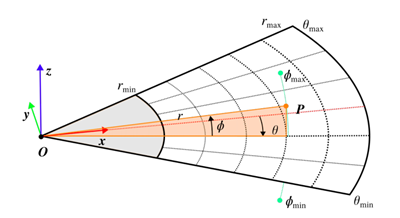
\includegraphics[width = 0.8\textwidth]{声纳成像1.png}
\caption{单个声纳图像的几何结构,点 $P$ 由范围 $r$、仰角 $\Phi$ 和方位角 $\theta$ 表示。\\
  $r_{\min}$, $r_{\max}$, $\Phi_{\min}$, $\Phi_{\max}$, $\theta_{\min}$, $\theta_{\max}$ 分别是成像声纳的最大和最小范围,\\
  最大仰角和最小仰角,最大方位角和最小方位角。}
\label{fig:声纳成像1}
\end{figure}

成像声纳通过发出一系列类似锥形的声波信号来生成部分球面测量值,从收发器测量观察到的反射信号的飞行时间,提供了反射表面的范围 $r$ 和方位角 $\theta$。但是这样的测量无法准确判断出
仰角 $\Phi$。因此,所有来自同一个方位角和距离的检测回波都会投影到声纳图像上的同一点 $I$( $\theta$, $r$),如图\ref{fig:声纳成像2}所示。对于对应于 $I$ 点中的某个方位角和距离
的像素,像素的强度对应于该方位角和距离下所有回波反射信号的强度。

\begin{figure}[ht]
	\centering
	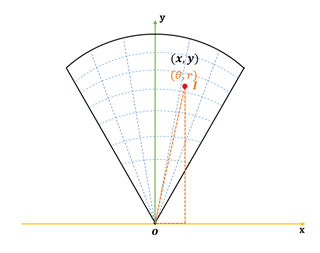
\includegraphics[width = 0.8\textwidth]{声纳成像2.png}
	\caption{真实声纳图像是整个垂直声纳数据在2D平面的投影。}
	\label{fig:声纳成像2}
\end{figure}

为了直观展示前视声纳的成像特征与其在水下环境感知中的应用,如图\ref{fig:水下机器人视觉图像与前视声纳图像对应示意图}所示,展示了同一时刻下水下机器人采集到的视觉图像与对应的前视
声纳图像。视觉图像反映了光学成像下的场景特征,可见由于水下光线传播的限制,视觉图像中的细节信息较为模糊。而前视声纳图像则通过声波反射捕捉了场景的结构信息,能够清晰地显示出障碍
物和地形特征。两者在信息维度和感知机制上存在显著差异。

\begin{figure}[!ht]
	\centering
	% ---- 定义标准尺寸盒子(以第一张图为基准)----
	\newsavebox{\standardbox}
	\savebox{\standardbox}{%
	  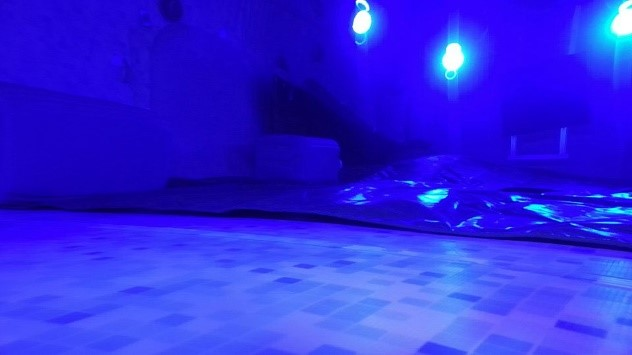
\includegraphics[width=0.47\textwidth]{figures/2-2视觉图像.jpg}%
	}
  
	% ---- 两张图并排,强制等宽等高 ----
	\begin{minipage}{\textwidth}
	  \centering
	  \subfigure[视觉图像\label{fig:2-2视觉图像}]{%
		\usebox{\standardbox}% 第一张:原始尺寸
	  }\hspace{0.5em}
	  \subfigure[前视声纳图像\label{fig:2-2声纳图像}]{%
		\resizebox{!}{\ht\standardbox}{% 强制等高
		  \resizebox{\wd\standardbox}{!}{% 强制等宽
			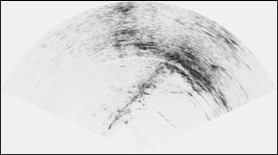
\includegraphics{figures/2-2声纳图像.jpg}%
		  }%
		}%
	  }
	\end{minipage}
  
	\caption{水下机器人视觉图像与前视声纳图像对应示意图}
	\label{fig:水下机器人视觉图像与前视声纳图像对应示意图}
  \end{figure}

需要指出的是,前视声纳图像通常可以以两种方式进行表示:一种是基于声纳测量参数,以方位角和距离为坐标轴的极坐标图像,直接对应于声纳的观测几何结构;另一种是通过坐标变换,
如公式\eqref{eq:coord}和\eqref{eq:polar}所示,将极坐标数据映射到笛卡尔平面上的笛卡尔坐标图像。前者能保留声纳探测的物理意义,后者则更便于与视觉图像进行对比以及后续的图像处理任务。
如图\ref{fig:笛卡尔与极坐标图像对应示意图}所示,左侧为前视声纳的笛卡尔图像,右侧为对应的极坐标图像。可以看出,笛卡尔图像通过坐标变换展现了空间中的物体分布,而极坐标图像则更直
观地展示探测的物体结构。

\begin{figure}[!ht]
	\centering
	\newsavebox{\leftpic}
	\savebox{\leftpic}{%
	  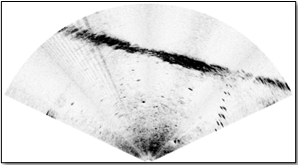
\includegraphics[height=4.1cm]{figures/笛卡尔图像.png}%
	}%

	% 左图
	\subfigure[前视声纳笛卡尔图像\label{fig:笛卡尔图像}]{%
	  \begin{minipage}[t]{\wd\leftpic}
	    \centering
	    \usebox{\leftpic}
	  \end{minipage}%
	}
	% 右图
	\subfigure[前视声纳极坐标图像\label{fig:极坐标图像}]{%
	  \begin{minipage}[t]{\wd\leftpic}
	    \centering
	    \resizebox{!}{\ht\leftpic}{%
	      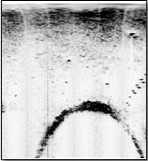
\includegraphics{figures/极坐标图像.jpg}%
	    }%
	  \end{minipage}%
	}%

	\caption{笛卡尔图像与极坐标图像对应示意图}
	\label{fig:笛卡尔与极坐标图像对应示意图}
\end{figure}


\section{循环一致性对抗网络}

循环一致性对抗网络(Cycle-Consistent Adversarial Network,CycleGAN)旨在解决图像到图像翻译的问题。该方法的核心在于能够在没有配对训练数据的情况下学习两个图像域之间的映射关系。对于
前视声纳这种缺少“干净”图像作为参考的情况,适合使用CycleGAN进行非配对图像去噪。传统图像翻译任务(如灰度图到彩色图、边缘图到照片)通常依赖于配对的输入和输出图像样本,但CycleGAN通过引
入循环一致性损失(Cycle Consistent loss),使其应用于许多实际场景,如艺术风格迁移,物体变形,季节转换和照片增强等。

图像到图像翻译的目标是将一个源域X中的图像转换为目标域Y中的图像。CycleGAN针对无配对设置,仅使用源域样本和目标域样本,通过对抗训练确保生成的图像分布与目标域匹配,并使用循环一致性避免模式崩溃。
CycleGAN的模型包含两个生成器和两个判别器。生成器 $G: X \rightarrow Y$ 将源域图像转换为目标域图像,生成器 $F: Y \rightarrow X$ 则执行相反的映射。判别器 $D_Y$ 旨在区分真实的目标域图像和
生成的图像,而判别器 $D_X$ 则区分真实的源域图像和生成的图像。这种双向对抗与映射结构如图\ref{fig:cyclegan1}所示,通过联合训练两个生成器和判别器,实现两个域之间的循环一致性翻译。

\begin{figure}[!ht]
	% 创建一个图形环境,[!ht] 表示优先将图形放置在“此处”或“页面顶部”
	\setlength{\subfigcapskip}{-1bp}
	% 设置子图标题与图像之间的间距为 -1bp(负值使标题更靠近图像)
	\centering
	% 使图形内容居中对齐
	\begin{minipage}{\textwidth}
	  % 创建一个宽度等于文本宽度的迷你页面,用于容纳子图
	  \centering
	  % 迷你页面内容居中
	  \subfigure[\label{fig:cyclegan1}]{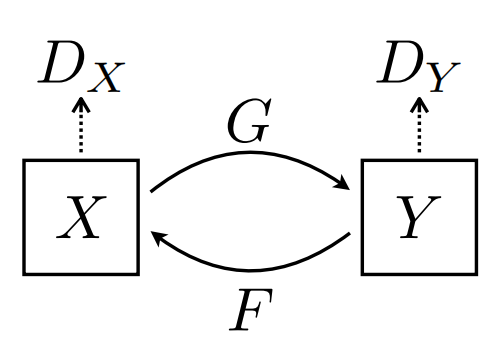
\includegraphics[width=0.3\textwidth]{figures/cyclegan1.jpg}}
	  % 定义第一个子图,标题为“图像1的标题”,插入图片 figures/1.jpg,宽度为文本宽度的 45%
	  \hspace{0.1em}
	  % 在两个子图之间添加 2em 的水平间距
	  \subfigure[\label{fig:cyclegan2}]{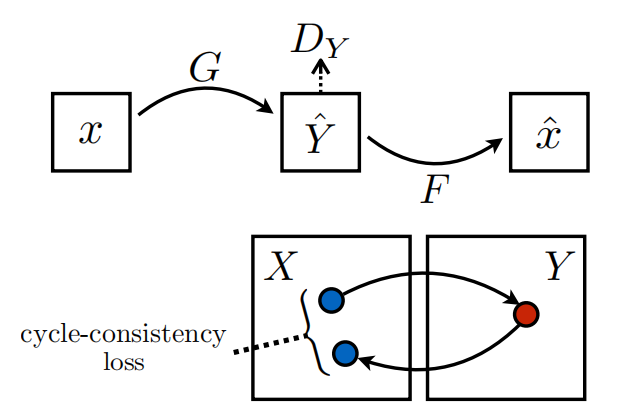
\includegraphics[width=0.3\textwidth]{figures/cyclegan2.jpg}}
	  \hspace{0.1em}
	  \subfigure[\label{fig:cyclegan3}]{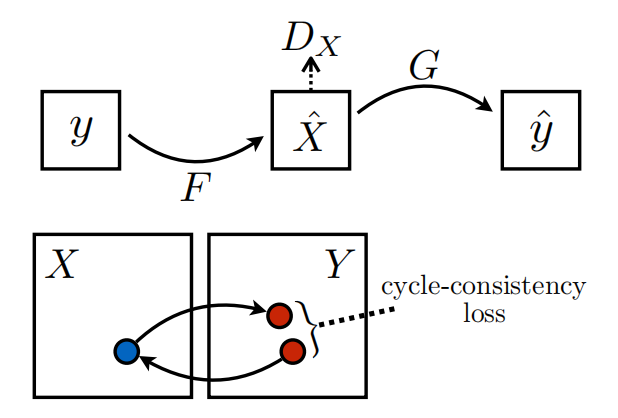
\includegraphics[width=0.3\textwidth]{figures/cyclegan3.jpg}}
	  % 定义第二个子图,标题为“图像2的标题”,插入图片 figures/2.jpg,宽度为文本宽度的 45%
	\end{minipage}
	% \vspace{0.2em}
	% 在图形与下方内容之间添加 0.2em 的垂直间距
	\caption{CycleGAN 示意图}
	\label{fig:cyclegan原理} % 为整个图形添加标签
  \end{figure}
  
为使生成器输出的图像在统计分布上与目标域相似,引入对抗损失函数。我们以$G: X \rightarrow Y$ 与判别器 $D_Y$ 为例,对抗损失 $\mathcal{L}_\mathrm{GAN}(G,D_Y,X,Y)$ 定义为:
\begin{equation}
    \label{eq1}
    \begin{aligned}
        \mathcal{L}_\mathrm{GAN}(G,D_Y,X,Y) &= \mathbb{E}_{y \sim p_Y}[\log D_Y(y)] \\
        &+ \mathbb{E}_{x \sim p_X}[\log (1-D_Y(G(x)))] 
    \end{aligned}.
\end{equation}
其中,$G$ 旨在生成足够“真实”的图像以欺骗判别器 $D_Y$,而 $D_Y$ 则尽力区分生成样本与真实样本。
同理,对抗损失 $\mathcal{L}_\mathrm{GAN}(F,D_X,Y,X)$ 对于 $F: Y \rightarrow X$ 及其对应的判别器 $D_X$ 也有类似的定义。
总对抗损失 $\mathcal{L}_{\mathrm{ad}}$ 是 $\mathcal{L}_\mathrm{GAN}(G,D_Y,X,Y)$ 和 $\mathcal{L}_\mathrm{GAN}(F,D_X,Y,X)$ 的加权和。

由于无配对训练样本无法保证 $x$ 与 $y$ 的一一对应,仅使用对抗损失会导致映射关系不稳定或模式坍塌。为此,CycleGAN引入循环一致性约束,要求经过双向映射的图像应该尽可能还原输入,
即:$F(G(x)) \approx x$ 和 $G(F(y)) \approx y$。相应的循环一致性损失函数定义为:
\begin{equation}
    \label{eq2}
    \begin{aligned}
        \mathcal{L}_\mathrm{cyc}(G,F) &= \mathbb{E}_{x \sim p_X}[\|F(G(x))-x\|_1] \\
        &+ \mathbb{E}_{y \sim p_Y}[\|G(F(y))-y\|_1] 
    \end{aligned}.
\end{equation}
如图\ref{fig:cyclegan2}和图\ref{fig:cyclegan3}所示,该约束确保跨域映射保留图像的结构信息,从而提升转换的一致性与可逆性。

在某些任务(如绘画到实景照片的风格迁移)中,CycleGAN可能在输入已经属于目标域时仍对图像进行不必要的颜色或亮度改变。为此,引入了身份映射损失,用于鼓励生成器在输入图像已经属于
目标域时保持输出不变。该损失函数定义如下:
\begin{equation}
    \label{eq3}
    \begin{aligned}
        \mathcal{L}_\mathrm{id}(G,F) &= \mathbb{E}_{y \sim p_Y}[\|G(y)-y\|_1] \\
        &+ \mathbb{E}_{x \sim p_X}[\|F(x)-x\|_1] 
    \end{aligned}.
\end{equation}
身份映射损失在保持图像色彩一致性与亮度分布方面具有重要作用,对于保护目标物体,防止去噪过多导致信息丢失尤为关键。

CycleGAN的总损失函数由上述三部分组成,损失函数如下:
\begin{equation}
    \label{eq4}
    \mathcal{L}(G, F, D_X, D_Y)=\mathcal{L}_{\mathrm{ad}}+\lambda_\mathrm{cyc}\,\mathcal{L}_\mathrm{cyc}(G,F)+\lambda_\mathrm{id}\,\mathcal{L}_\mathrm{id}(G,F).
\end{equation}
其中,$\lambda_{cyc}$ 与 $\lambda_{id}$ 分别为循环一致性与身份损失的权重系数。最终优化目标为:
\begin{equation}
	\label{eq5}
	G^*, F^* = \arg \min_{G,F} \max_{D_X, D_Y} \mathcal{L}(G, F, D_X, D_Y).
\end{equation}


\section{循环一致性对抗网络}

循环一致性对抗网络(Cycle-Consistent Adversarial Network,CycleGAN)由 Zhu 等人于 2017 年提出~\cite{zhu2017unpaired},旨在解决无配对条件下的图像到图像翻译问题(Unpaired Image-to-Image Translation)。
与传统的监督式方法(如 Pix2Pix~\cite{isola2017image})不同,CycleGAN 能在没有配对训练数据的情况下学习两个图像域之间的映射关系。
这一特性使其特别适用于缺乏“干净”参考图像的场景,例如前视声纳图像去噪任务中,真实环境下几乎不可能同时获得同一场景的有噪声与无噪声配对图像。

传统的图像翻译任务(如灰度图到彩色图、素描到照片、昼夜转换等)往往依赖成对的训练样本 $(x_i, y_i)$。
而在声纳成像等非理想观测条件下,配对样本的获取代价极高甚至无法实现。
CycleGAN 通过引入循环一致性约束(Cycle Consistency Loss)与身份映射约束(Identity Loss),在保证结构一致性的同时实现了跨域映射学习,为非配对图像去噪提供了一种高效的可行方案。

CycleGAN 的整体结构包含两个生成器(Generator)和两个判别器(Discriminator),分别建立在两个域 $X$ 和 $Y$ 之间的对偶映射关系:
生成器 $G: X \rightarrow Y$ 将源域图像转换为目标域风格,生成器 $F: Y \rightarrow X$ 执行逆向映射。
判别器 $D_Y$ 用于判别输入图像是否来自目标域 $Y$,而 $D_X$ 判别输入图像是否属于源域 $X$。
这种双向的对抗结构如图~\ref{fig:cyclegan1} 所示,通过相互约束与循环反馈,使得生成的图像在语义与结构上保持一致。

\begin{figure}[!ht]
	% 创建一个图形环境,[!ht] 表示优先将图形放置在“此处”或“页面顶部”
	\setlength{\subfigcapskip}{-1bp}
	% 设置子图标题与图像之间的间距为 -1bp(负值使标题更靠近图像)
	\centering
	% 使图形内容居中对齐
	\begin{minipage}{\textwidth}
	  % 创建一个宽度等于文本宽度的迷你页面,用于容纳子图
	  \centering
	  % 迷你页面内容居中
	  \subfigure[\label{fig:cyclegan1}]{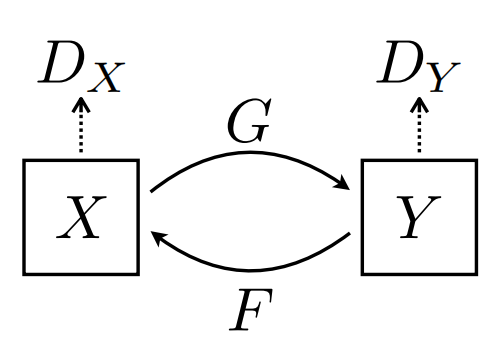
\includegraphics[width=0.3\textwidth]{figures/cyclegan1.jpg}}
	  % 定义第一个子图,标题为“图像1的标题”,插入图片 figures/1.jpg,宽度为文本宽度的 45%
	  \hspace{0.1em}
	  % 在两个子图之间添加 2em 的水平间距
	  \subfigure[\label{fig:cyclegan2}]{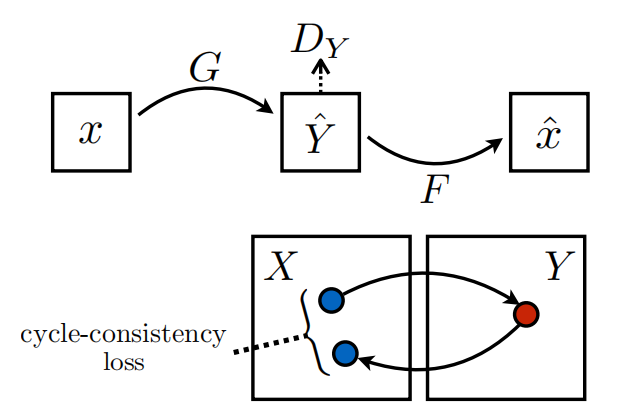
\includegraphics[width=0.3\textwidth]{figures/cyclegan2.jpg}}
	  \hspace{0.1em}
	  \subfigure[\label{fig:cyclegan3}]{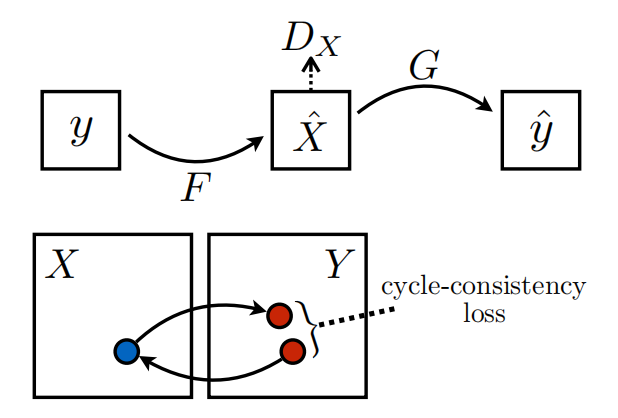
\includegraphics[width=0.3\textwidth]{figures/cyclegan3.jpg}}
	  % 定义第二个子图,标题为“图像2的标题”,插入图片 figures/2.jpg,宽度为文本宽度的 45%
	\end{minipage}
	% \vspace{0.2em}
	% 在图形与下方内容之间添加 0.2em 的垂直间距
	\caption{CycleGAN 示意图}
	\label{fig:cyclegan原理} % 为整个图形添加标签
  \end{figure}

在网络设计上,CycleGAN 的生成器采用了基于 U-Net~\cite{ronneberger2015u} 或 ResNet~\cite{johnson2016perceptual} 的结构,以便在跨域变换中保留低层特征与高层语义信息。
其中,ResNet 生成器通常由 $9$ 个残差块(Residual Blocks)组成,以捕获复杂的跨域映射特征。
判别器则采用 PatchGAN~\cite{isola2017image} 结构,通过判断每个局部图像块的真假性来提高模型的细节保真度,从而生成更自然、更逼真的图像纹理。

为确保生成图像在分布上接近目标域,CycleGAN引入了对抗损失函数。以 $G: X \rightarrow Y$ 与判别器 $D_Y$ 为例,其对抗损失定义如下:
\begin{equation}
    \label{eq1}
    \begin{aligned}
        \mathcal{L}_\mathrm{GAN}(G,D_Y,X,Y) &= \mathbb{E}_{y \sim p_Y}[\log D_Y(y)] \\
        &+ \mathbb{E}_{x \sim p_X}[\log (1-D_Y(G(x)))].
    \end{aligned}
\end{equation}
生成器 $G$ 旨在生成足够真实的图像以欺骗判别器 $D_Y$,而判别器 $D_Y$ 则学习区分真实样本与伪造样本。
同理,对于 $F: Y \rightarrow X$ 及其对应的判别器 $D_X$,定义类似的损失项 $\mathcal{L}_\mathrm{GAN}(F,D_X,Y,X)$。
两者之和构成总对抗损失 $\mathcal{L}_\mathrm{ad}$。

由于无配对训练样本无法保证 $x$ 与 $y$ 的一一对应,仅靠对抗训练容易导致模式坍塌(Mode Collapse)或结构失真。
为约束生成器学习稳定的可逆映射关系,CycleGAN 引入循环一致性损失,要求经过双向映射的图像尽可能还原输入:
\[
F(G(x)) \approx x, \quad G(F(y)) \approx y.
\]
循环一致性损失定义为:
\begin{equation}
    \label{eq2}
    \begin{aligned}
        \mathcal{L}_\mathrm{cyc}(G,F) &= \mathbb{E}_{x \sim p_X}[\|F(G(x))-x\|_1] \\
        &+ \mathbb{E}_{y \sim p_Y}[\|G(F(y))-y\|_1].
    \end{aligned}
\end{equation}
该项损失确保模型在跨域转换过程中保留图像的几何与结构特征,提升了生成结果的稳定性与可逆性。
在声纳图像去噪任务中,该约束有助于保持场景目标的空间一致性,避免在去噪过程中出现结构模糊或物体形态扭曲。

在部分任务(如绘画到实景照片或光照增强)中,若输入图像本身已经接近目标域,模型可能在不必要的情况下改变色彩或亮度。
为缓解这一问题,引入身份映射损失(Identity Loss)以约束生成器的输出应尽量保持与输入一致:
\begin{equation}
    \label{eq3}
    \begin{aligned}
        \mathcal{L}_\mathrm{id}(G,F) &= \mathbb{E}_{y \sim p_Y}[\|G(y)-y\|_1] \\
        &+ \mathbb{E}_{x \sim p_X}[\|F(x)-x\|_1].
    \end{aligned}
\end{equation}
该项损失在保持图像色彩与亮度一致性方面具有显著作用。
在声纳去噪任务中,身份约束可以防止生成器过度平滑目标结构,防止噪声抑制导致的细节丢失。

CycleGAN 的整体优化目标由三部分损失组成:
\begin{equation}
    \label{eq4}
    \mathcal{L}(G, F, D_X, D_Y)=\mathcal{L}_{\mathrm{ad}}+\lambda_\mathrm{cyc}\,\mathcal{L}_\mathrm{cyc}(G,F)+\lambda_\mathrm{id}\,\mathcal{L}_\mathrm{id}(G,F),
\end{equation}
其中,$\lambda_\mathrm{cyc}$ 与 $\lambda_\mathrm{id}$ 分别为循环一致性与身份损失的权重系数。
原论文中通常取 $\lambda_\mathrm{cyc}=10$,$\lambda_\mathrm{id}=0.5\,\lambda_\mathrm{cyc}$。
最终优化目标为:
\begin{equation}
	\label{eq5}
	G^*, F^* = \arg \min_{G,F} \max_{D_X, D_Y} \mathcal{L}(G, F, D_X, D_Y).
\end{equation}

CycleGAN 的核心优势在于其无监督学习特性与结构保持能力:
\begin{itemize}
    \item 不依赖配对样本即可实现跨域映射;
    \item 保留源图像的几何结构与语义一致性;
    \item 可扩展性强,适用于风格迁移、图像增强、语义分割前处理等多种任务。
\end{itemize}
在前视声纳图像去噪任务中,CycleGAN 能够学习噪声域与干净域之间的隐式映射关系,通过对抗学习抑制随机噪声,同时依靠循环一致性与身份约束保持目标结构完整。
这为后续的结构性噪声抑制提供了可靠的先验。





\section{声纳图像无配对去噪网络的构建与优化}
本研究中,声纳图像的噪声域和干净域分别由含噪声的真实声纳图像和通过模拟仿真生成的声纳图像构成。由于实际采集的声纳图像往往受到环境和设备因素影响而包含复杂噪声,而仿真生成的图像可以在理想条件下
生成,具有较高的结构与纹理清晰度,因此两者在视觉特性上存在明显域差异。为了在无配对条件下实现这两种域间的特征迁移,本阶段采用CycleGAN为核心框架,构建噪声域到干净域,干净域到噪声域的双向映射,
通过循环一致性约束实现结构信息的保持与伪影的抑制。

\begin{figure}[ht]
	\centering
	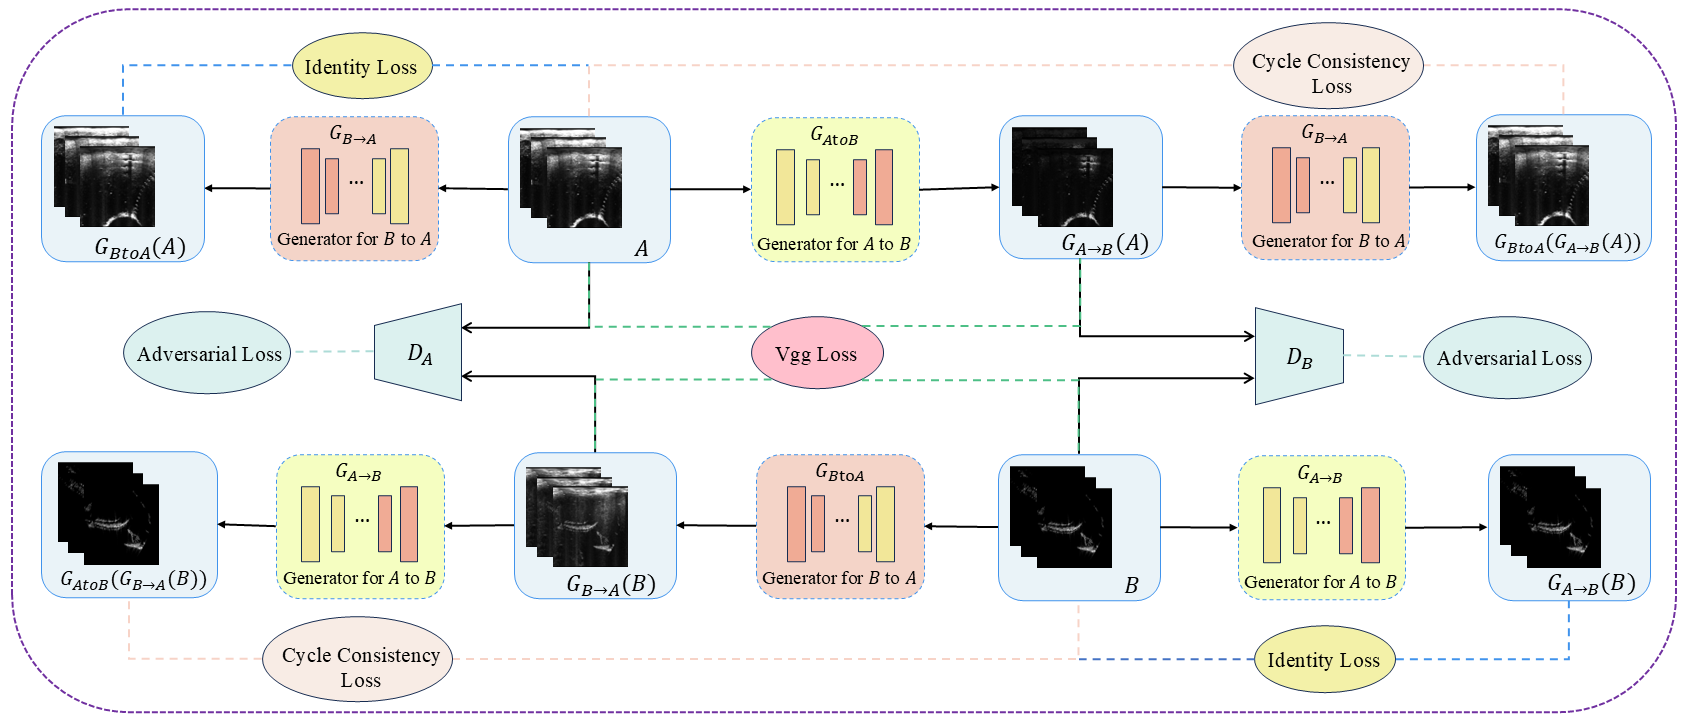
\includegraphics[width = 1.0\textwidth]{upd1.png}
	\caption{}
	\label{fig:upd1}
\end{figure}
	

